\documentclass{homework}
\usepackage{enumitem}
\author{Kitty Wang}
\class{Thermodynamics and Climate Change\newline Professor P. Godart}
\date{\today}
\title{Problem Set 1}

\graphicspath{{./media/}}

\begin{document} \maketitle

\question Properties of a thermodynamic system
\begin{enumerate}[label=(\alph*)]
\item The temperature of the water is an intensive property of the thermodynamic system as it is a measurable quantity at any given time, and is not dependent on the history of the system.
\item Similar to temperature, the density of the water is also an intensive property of the system because it depends only on the state of the system and does not consider the system’s history.
\item The amount of water exchanged with lower layers each month cannot be classified as a thermodynamic property since it requires the summation of the exchange of water over an interval of time, and thus is dependent on the history of the system.
\item The concentration of dissolved oxygen in the water is an intensive property of the system because it can be measured at a given time, and assumes a definite, exact value when the system is in a particular state. Because the concentration of dissolved $\mathf{O_2}$ is also independent of the system size and may vary from place to place within the system at any moment, it can be considered an intensive property.
\item Likewise, the atmospheric pressure at the water’s surface is also an intensive property of the system as it is a measurable quantity at a particular moment in the system and depends only on the given state of the system.
\item The concentration of salt in the water is an intensive property of the system since its value does not fluctuate with the system’s scale and takes on a definite value when the system is in a specific state.
\item Similar to part(c), the amount of water that evaporates each day is not a property of the system because it relies on the processes connecting multiple states of the system and requires the summation of the amount of water evaporated over a duration of time. Thus, it is not dependent only on the state of the system.
\end{enumerate}

\question Concept Questions
\begin{enumerate}[label=(\alph*)]
    \item For the following, state the type(s) and method of energy conversion (e.g. mechanical to thermal via frictional dissipation):
    \begin{enumerate}[label=\roman*.]
        \item A block sliding down an inline and coming to stop experiences a conversion of mechanical to thermal energy via frictional dissipation.
        \item Rain falling from a cloud and hitting the ground experiences a conversion of potential energy into kinetic energy as it is falling due to gravitational forces. Some of the energy is also converted into thermal energy as the raindrops hit the ground.
        \item The ground heating up in the sun experiences an energy transformation of solar to thermal energy via absorption.
        \item A forest fire sees the conversion between chemical energy into thermal energy via combustion.
        \item Ice melting experiences the energy conversion from thermal energy into potential energy via absorption.
        \item Air expanding as it is heated see a transformation between thermal to kinetic energy. The thermal energy increases the speed of the gas particles within the air. The increased kinetic energy of the gas particles then results in a volume increase.
    \end{enumerate}
    \item For an ideal gas at constant pressure:
    \begin{enumerate}[label=\roman*.]
        \item Based on the ideal gas law, the volume increases proportionally with an increase in temperature, similar to the case made in Question 2(a)(vi).
        \item The volume decreases by half if one removes half of the molecules of gas to balance out PV and nRT in the ideal gas law.
        \item It would require more energy to achieve the same temperature than if the gas was kept at constant volume because at constant volume, all of the heat added contributes directly to increasing the temperature, as opposed to being allocated toward expanding the volume.
    \end{enumerate}
    \item In which of the following cases is the First Law of Thermodynamics violated?
    \begin{enumerate}[label=\roman*.]
        \item A solar sail in outer space that accelerates by sunlight shining on adheres to the First Law of Thermodynamics because the sun is constantly supplying the energy required to perform the work necessary for the transformation of solar energy into mechanical energy for the apparatus to accelerate. Energy is not created or destroyed, but rather converted into different forms to power the solar sail, and light has momentum.
        \item A balloon that rises when you heat the gas inside also abides by the First Law of Thermodynamics since the total energy contained within the closed system remains constant, and the thermal energy expended by the heat source transforms into an alternate form of energy — the kinetic energy of the gas particles within the balloon. The increased kinetic energy of the gas particles then results in a volume increase that causes a lower density for the balloon to rise.
        \item A block sliding on a frictional surface without slowing down violates the First Law of Thermodynamics because the change in internal energy induced by the frictional forces is generated from the thermal energy transferred. The converted thermal energy must slow down the block to conserve the total energy.
        \item A device that extracts mechanical work from a heated block without cooling the block down also violates the First Law of Thermodynamics because the process of extracting energy from the heated block as heat requires a temperature decrease and general change, which would induce cooling in the block.
        \item The Moon causing tides on Earth aligns with the First Law of Thermodynamics because the changes in gravitational potential energy and the rotational kinetic energy of the Earth provide the energy input to create tides on the planet. However, as this energy is dissipated by friction, the Earth’s rotation will slow and eventually become tidally locked.
    \end{enumerate}
    \item 
    \begin{enumerate}[label=\roman*.]
        \item Ice absorbs thermal energy as it melts as it must gain energy to break the bonds holding the ice molecule structure together through latent heat.
        \item Water also absorbs thermal energy as it evaporates because its gaseous state requires more kinetic energy to increase the speed of the particles.
    \end{enumerate}
\end{enumerate}


\question A Earth without its atmosphere
\begin{enumerate}[label=(\alph*)]
    \item
    From the First Law of Thermodynamics, it is given that:
    \begin{center}$\mathf{E_2} - \mathf{E_1} = \mathf{Q} - \mathf{W}$
    \end{center}
    Given two states that are arbitrarily close in time to each other, we can implicitly differentiate both sides' expression with respect to time. This process yields
    \begin{center}$\mathf{\dot E_{CV}} = \mathf{\dot Q} - \mathf{\dot W}$\end{center}
    Since no work is performed within the control volume, the term representing work may be eliminated and the equation can be rewritten as
    \begin{center}$\mathf{\dot Q_{in}} = \mathf{\dot Q_{out}}$
    \end{center}
    Because $\mathf{\dot Q_{in}}$ is defined by $\mathf{\dot q"_{solar}}$ and $\mathf{\dot Q_{out}}$ is defined by $\mathf{\dot q"_{radiated}}$, assuming radiative equilibrium, we can reframe the above to an equivalence of the power absorbed by the Earth and the power radiated by the Earth to space. Suppose the solar rays form a parallel beam of light, and the earth intercepts a surface area equal to $\mathf{R_e^2\pi}$, using some unit conversion and the Stefan-Boltzmann law, we can express this equation as
    \begin{center}
        $\mathf{(1 - a) E_e{R_e^2\pi}} =\mathf{\varepsilon\sigma(4{R_e^2\pi})T^4}$
    \end{center}
   \begin{center}
       Eliminating the $\mathf{R_e^2\pi}$ term on both sides yields
   \end{center} 
    \begin{center}
        $\mathf{(1 - a)E_e} = \mathf{4\varepsilon\sigma T^4}$
    \end{center}
    where $\mathf{a}$ represents albedo, $\mathf{E_e}$ is irradiance, $\mathf{\varepsilon}$ represents emissivity, $\mathf{\sigma}$ is the Stefan-Boltzmann constant, and $\mathf{T}$ is the temperature of the Earth's surface. Substituting the question's given quantities yields
    \begin{center}
        $\mathf{(1 - 0.3)(1400\frac{W}{m^2})} =\mathf{4(0.8)(5.67\cdot 10^{-8}\frac{W}{m^2K^4})T^4}$
    \end{center}
    \begin{center}
        $\mathf{T^4 = \frac{(0.7)(1400\frac{W}{m^2})}{4(0.8)(5.67\cdot 10^{-8}\frac{W}{m^2K^4})}}$
    \end{center}
    \begin{center}
        $\mathf{T^4 = 5.40123 \cdot 10^{9}}$K\textsuperscript{4}
    \end{center}
    \begin{center}
        $\mathf{T = 271.096}$ K
    \end{center}
    Therefore, the estimated temperature of the Earth's surface is 271.1 K, or -2.05$^{\circ}$C.
    \item My calculated value of -2.05$^{\circ}$C is higher than the more detailed computer simulation approximation of -18${^\circ}$C. This may be attributed to the difference in the angle of incidence of the sunlight beam, which may result in a discrepancy in the irradiance used. In addition, physical structures on the earth such as mountains may cast shadows.
\end{enumerate}

\question Energy lost in a spring
\begin{enumerate}[label={(\alph*)}]
    \item 
    If the spring was ideal and follows the First Law of Thermodynamics, then the change in energy between two states is equal to the difference between the heat transferred and the work done by the system. This can be expressed as 
    \begin{center}$\mathf{E_2} - \mathf{E_1} = \mathf{Q} - \mathf{W}$
    \end{center}
    Because the spring does not dissipate any energy, no heat is transferred between the system and its environment, thus yielding
    \begin{center}$\mathf{\Delta E} = - \mathf{W}$
    \end{center}
    \begin{center}
        where $\mathf{Q}$ can be eliminated as it evaluates to 0.0 J.
    \end{center}
    \begin{center}
        $\mathf{\therefore \Delta E = - W = \Delta PE_s}$
    \end{center}
    since all of the work done by the subject will be converted into spring potential energy. As we have derived both in and out of class, spring potential energy can be expressed as 
    \begin{center}
        $\mathf{\Delta PE_s = \frac{1}{2}kx^2}$
    \end{center}
    Substituting the given quantities yields the following simplified equation
    \begin{center}
        $\mathf{\Delta PE_s = -\frac{1}{2}(750\frac{N}{m})(0.1 m)^2}$ 
    \end{center}
    \begin{center}
        and
    \end{center}
     \begin{center}
        $\mathf{W = \Delta PE_s = 3.75}$ J 
    \end{center}
    \item 
    In the process with the non-ideal spring, some thermal energy dissipated in the process of compression. We can begin again from the equation provided under the First Law of Thermodynamics:
    \begin{center}$\mathf{E_2} - \mathf{E_1} = \mathf{Q} - \mathf{W}$
    \end{center}
     \begin{center}$\mathf{\Delta E} = \mathf{Q} - \mathf{W}$
    \end{center}
    From part(a), we have computed the energy for work expended under an ideal case, so we can substitute this value, along with the given quantity for the empirical 5 J of work put in, as the work and change in total energy, respectively.
    \begin{center}
        $\mathf{3.75 J = Q - (- 5 J)}$
    \end{center}
    \begin{center}
        $\mathf{\therefore Q = -1.25 J}$
    \end{center}
    \item If the spring is made of iron and has a mass of 5kg, we can calculate the temperature using the equation 
    \begin{center}
         $\mathf{Q = mc\Delta T}$
    \end{center}
    
        Given that iron has a specific heat capacity of 444 J/kg-K, we can substitute this as the c value in addition to the computed Q quantity from part(b), which yields
    \begin{center}
         $\mathf{1.25 J = (5 kg)(444 J/kg\cdot K)(\Delta T)}$
    \end{center}
    \begin{center}
        $\mathf{\Delta T = 5.63 \cdot 10^{-4}}$ K
    \end{center}



\end{enumerate}
\question Challenge: Atmospheric pressure
\begin{center}
    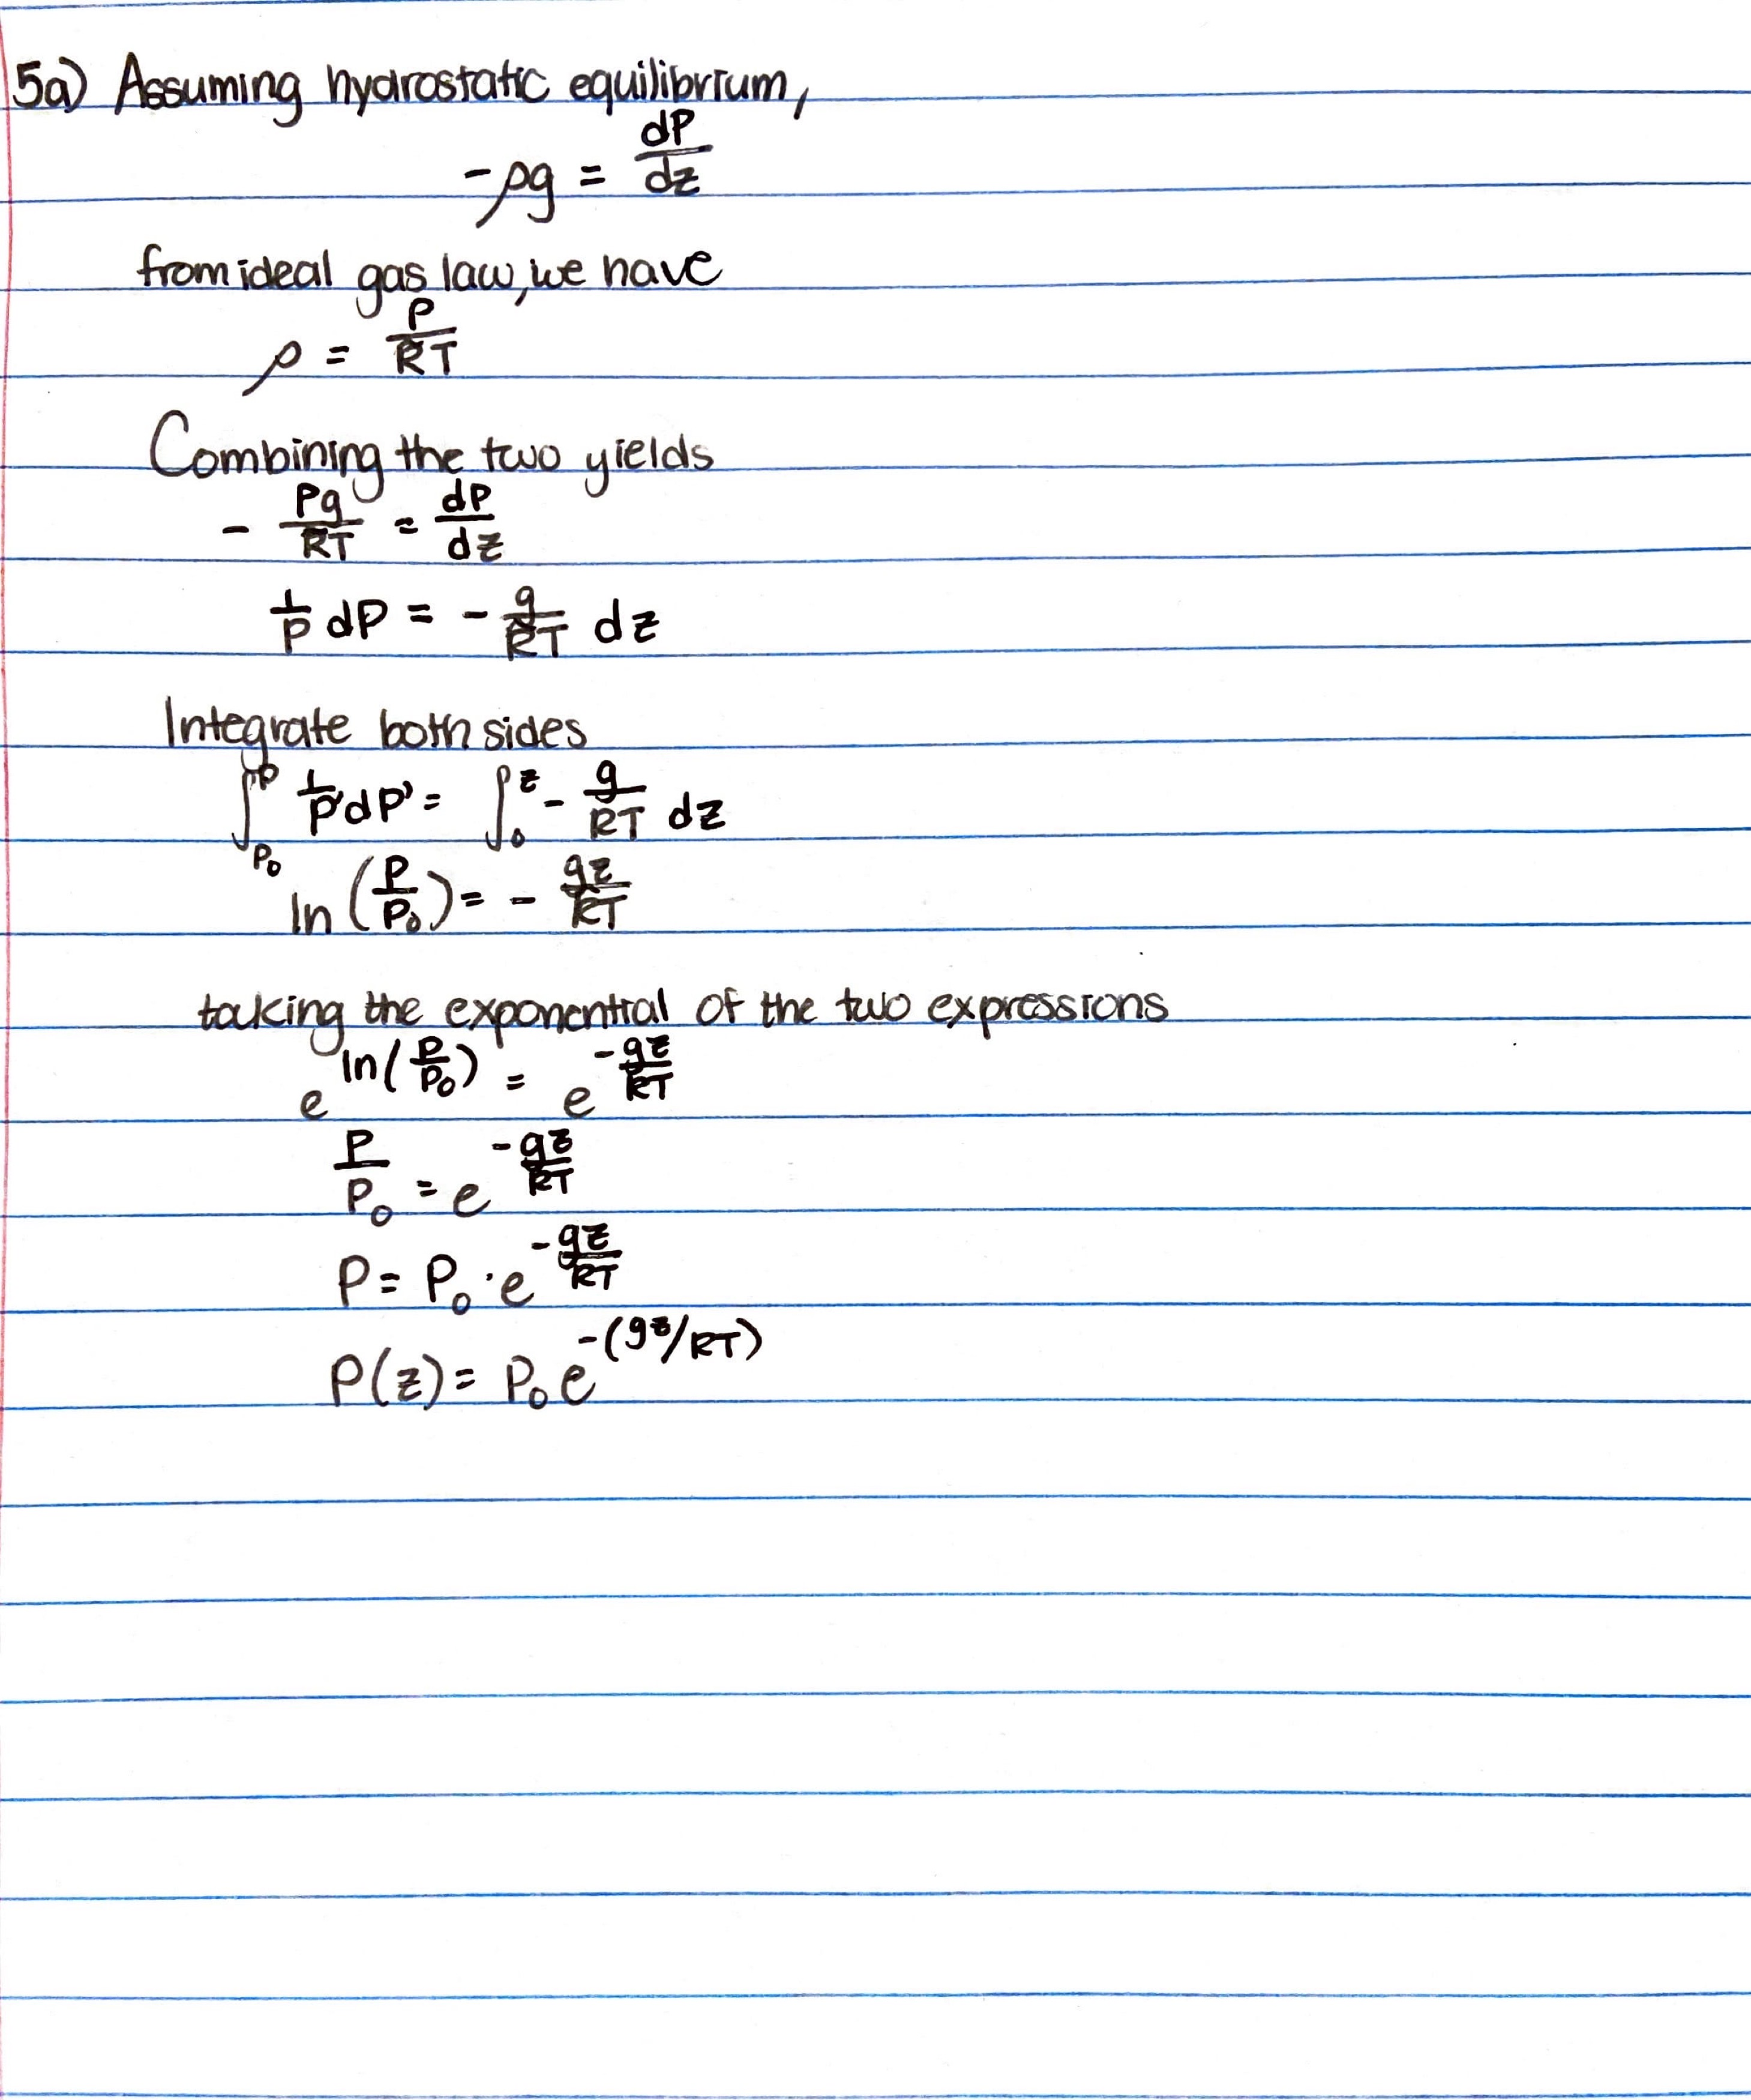
\includegraphics[width=15cm]{media/5a.JPG}
\end{center}
\begin{center}
    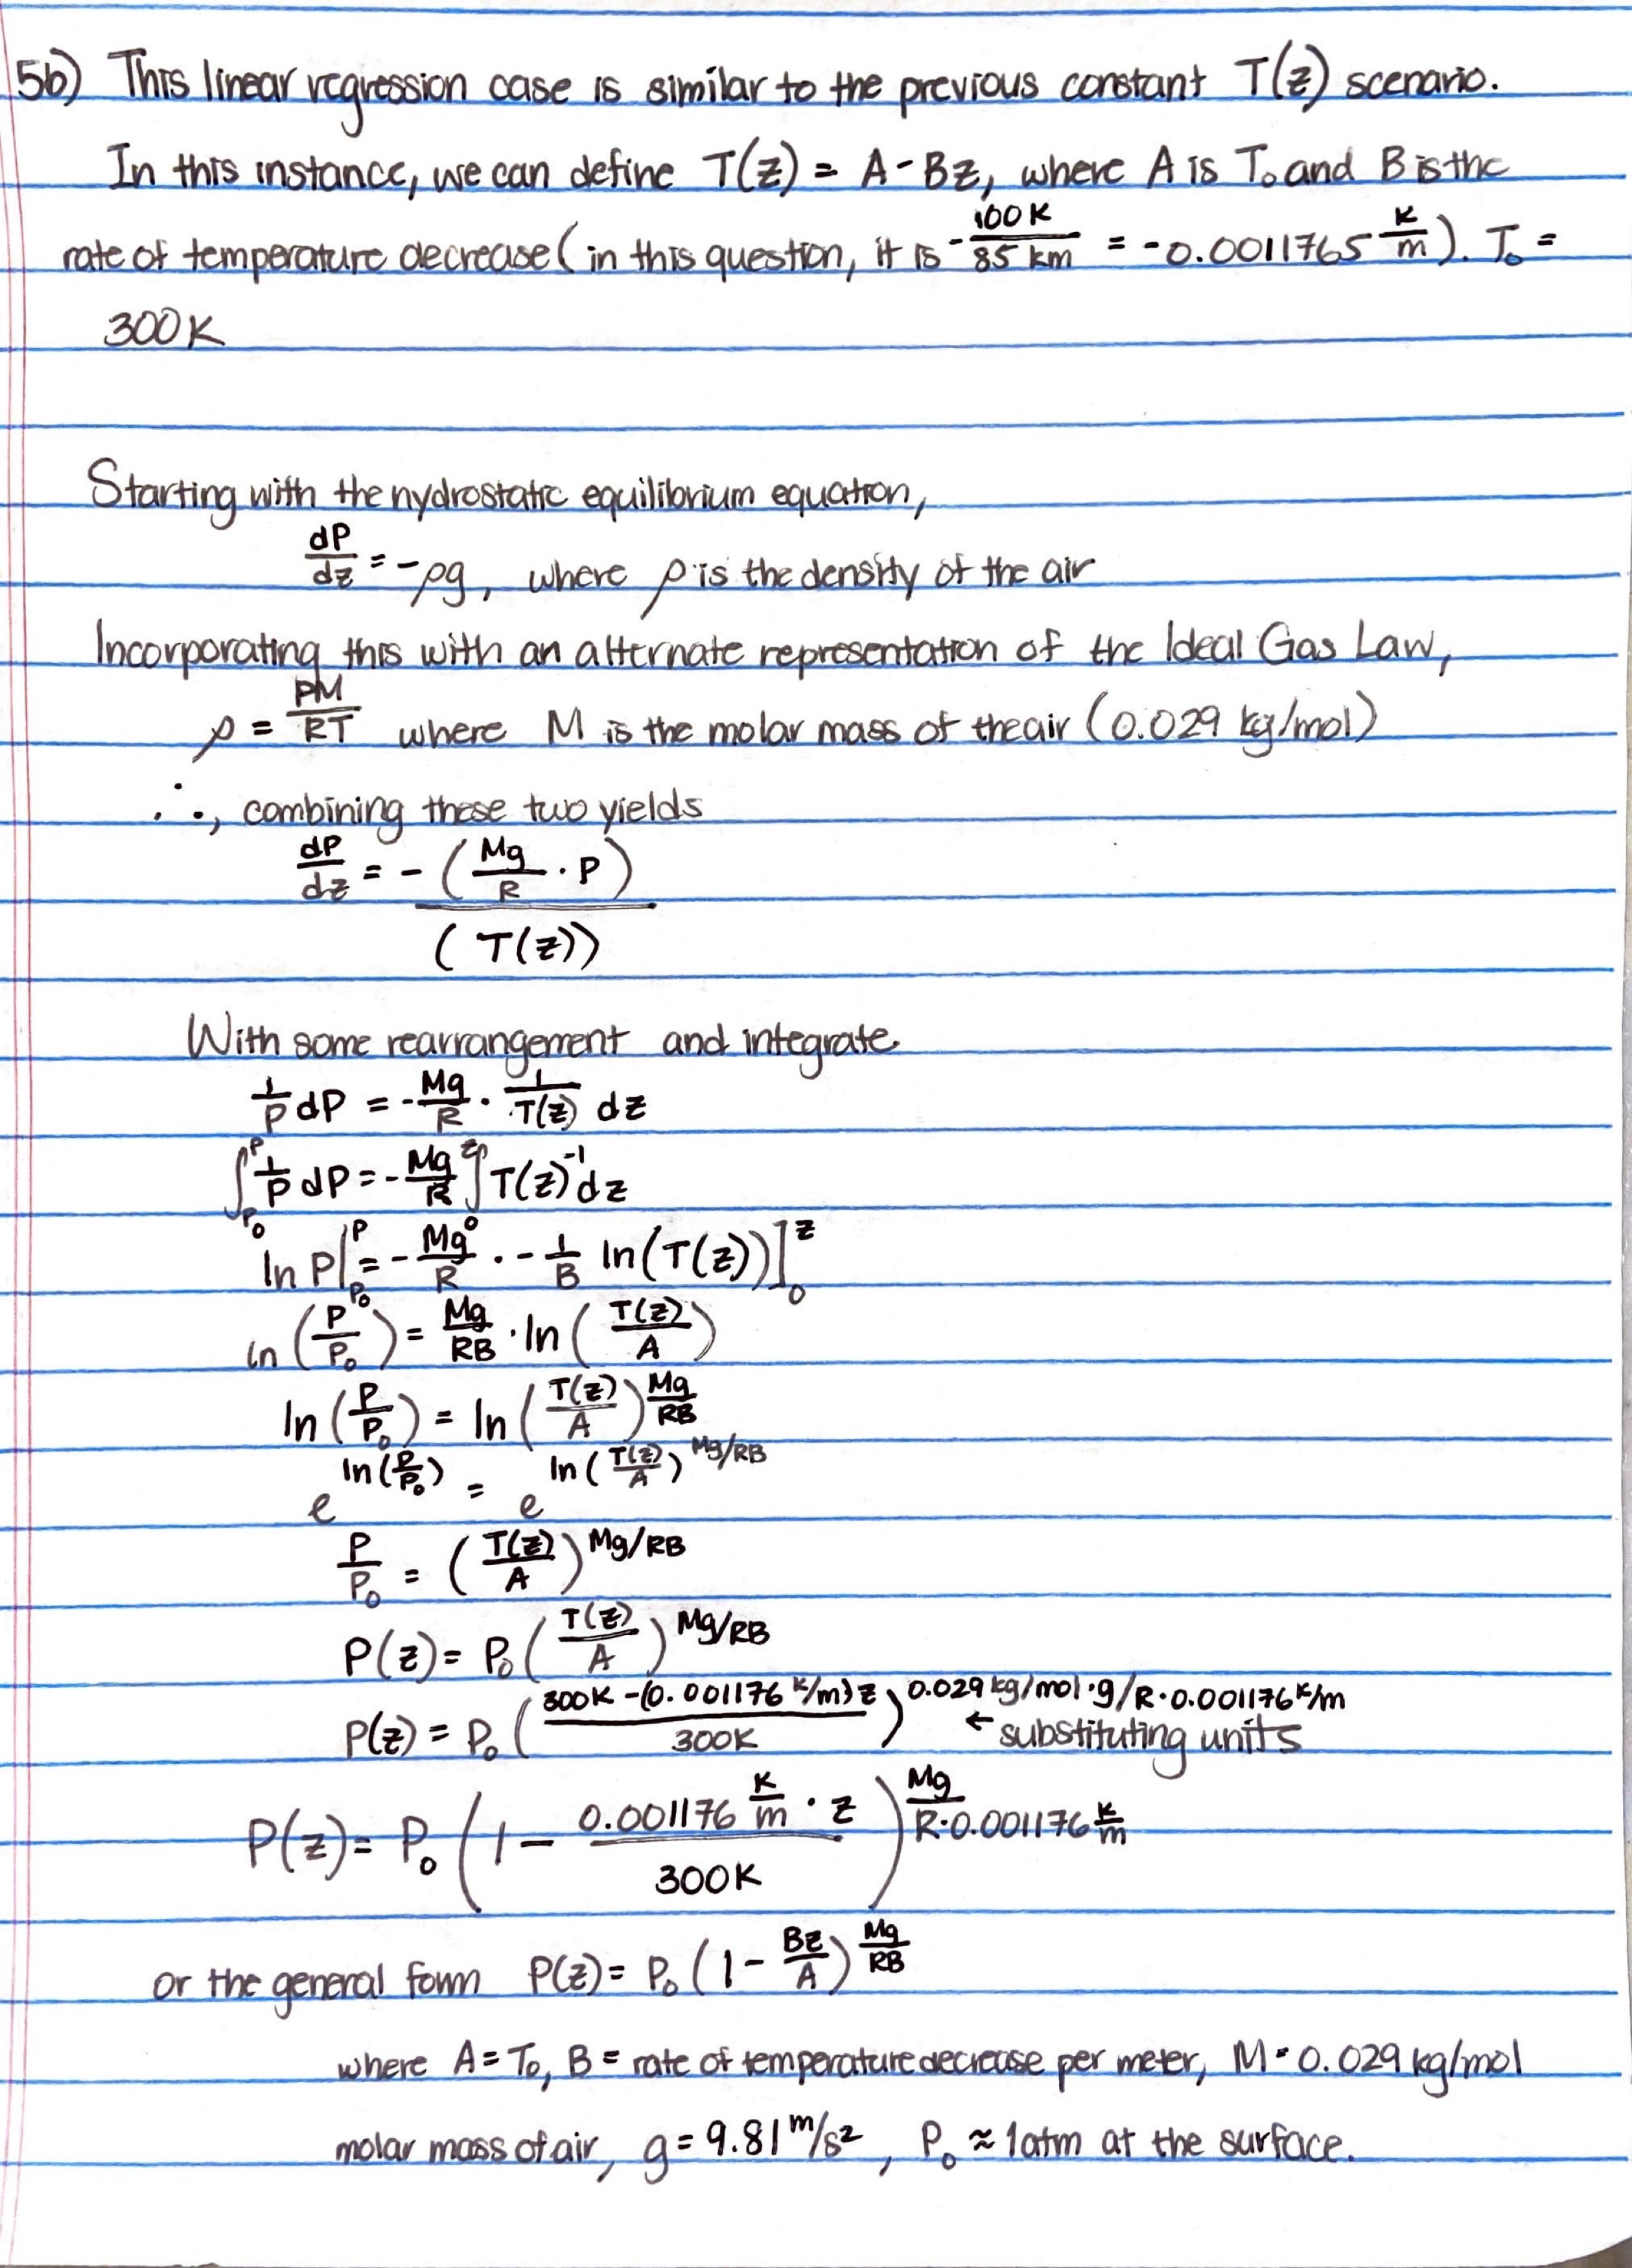
\includegraphics[width=15cm]{media/5b.JPG}
\end{center}
\begin{center}
    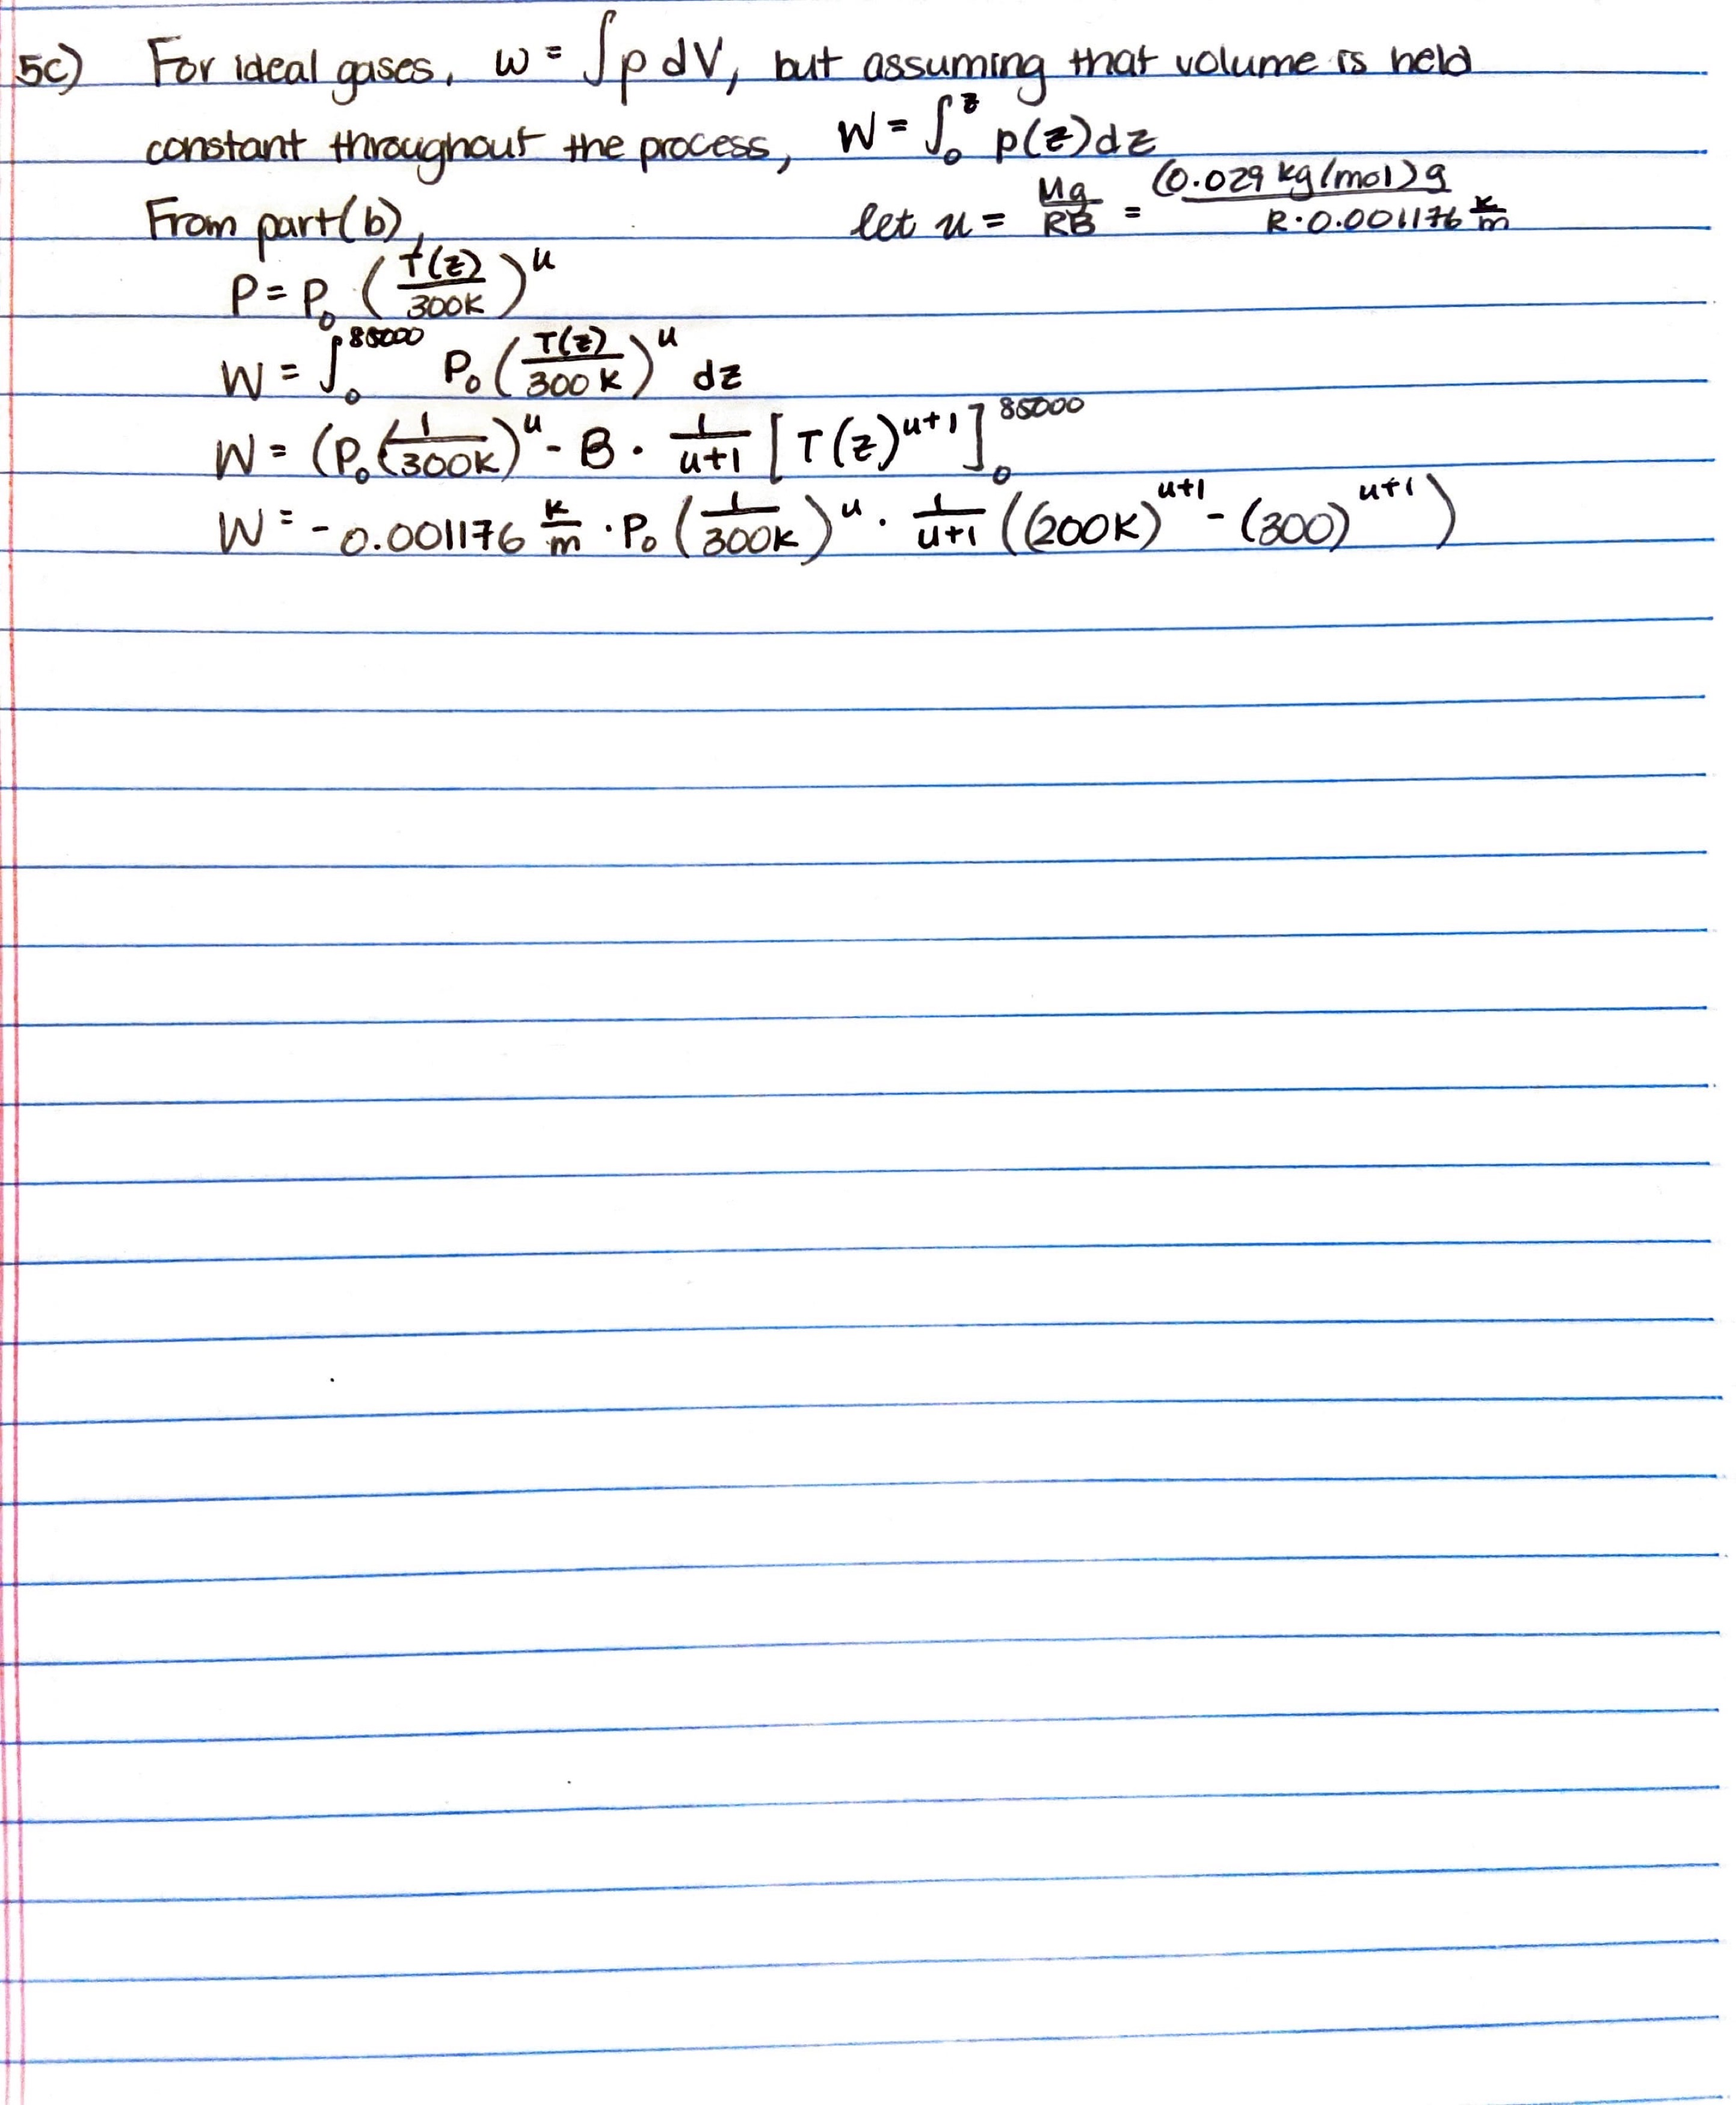
\includegraphics[width=15cm]{media/5c.JPG}
\end{center}


% citations
% \bibliographystyle{plain}
% \bibliography{citations}

\end{document}